% Chapter2

\chapter{State of the Art} \label{chapter:stateoftheart}

	% ##################################################################
	% Warum welche Hardware (Kriterien für unsere Nutzung, Umsetzbarkeit
	% ##################################################################
	\section{Hardwareaufbau einer SPS}
	
	Um die im späteren Verlauf darauf aufbauende Hardware genauer beschreiben zu können, muss zu Beginn ein wenig thematisch ausgeholt werden. So hat der Begriff der Steuerung einen undenkbar hohen Stellenwert, welcher ebenso geklärt gehört.\\
	
	Unter einer Steuerung eines Prozesses versteht man nach der standardisierten Norm DIN 19226 einen Vorgang, bei dem durch Rückführen gemessener Prozesszustände, verglichen mit von der speicherprogrammierbaren Steuerung formulierten Parametern, Sollwerte zur Beeinflussung des gesamten Prozesses erzeugt werden. Im Gegensatz zu einer Regelung, muss der von einem Sensor ausgelesene Ist-Wert jedoch nicht zwanghaft rückgeführt werden.\\
	
	\begin{figure}[h!]
  		\centering
      	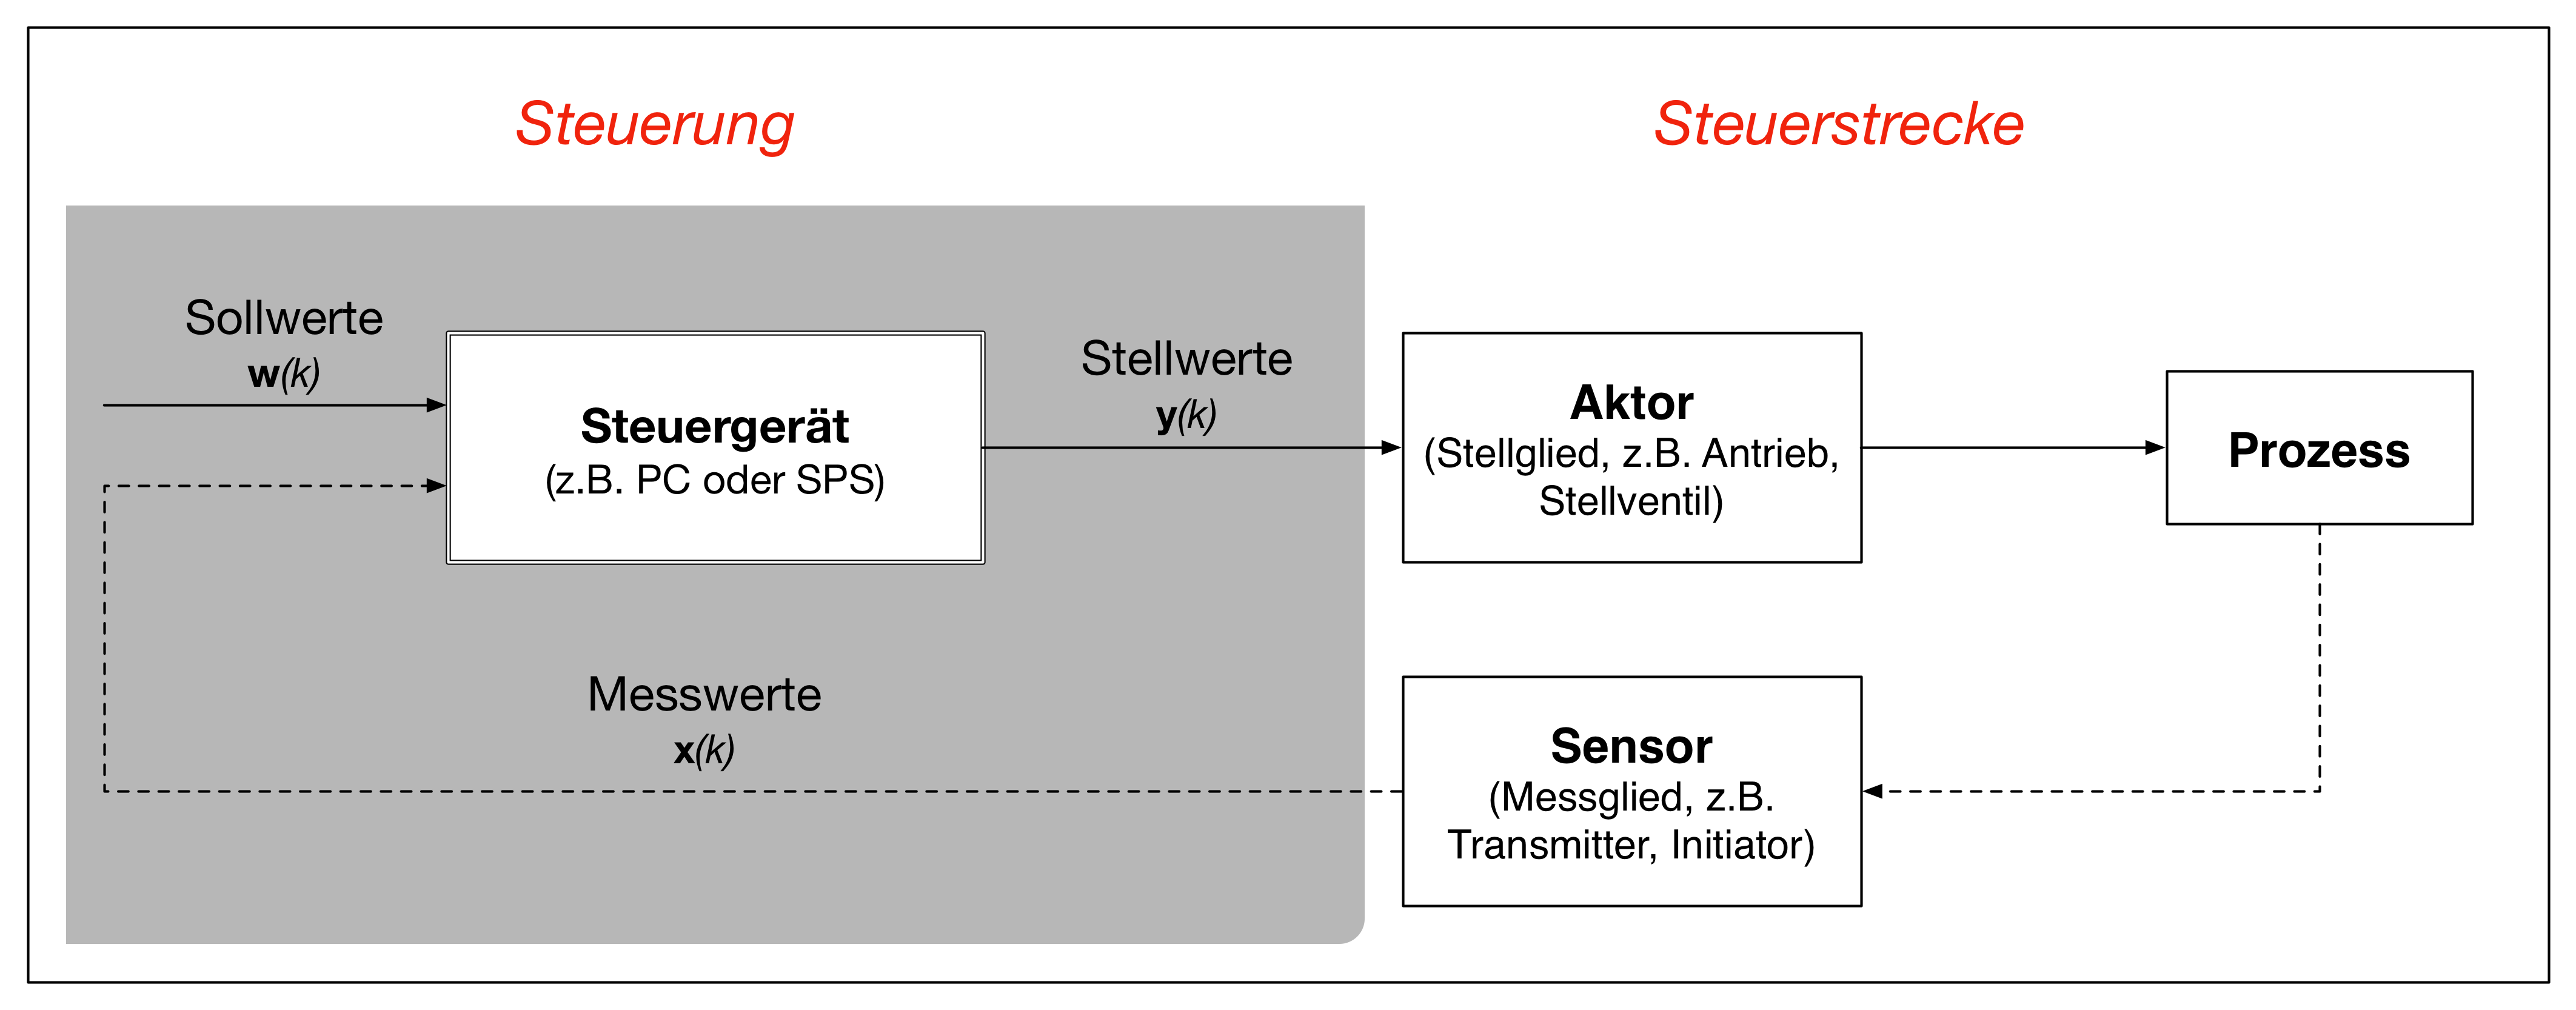
\includegraphics[width=0.8\textwidth]{graphics/stateoftheart/Aufbau_Steuerkreis_Selfmade.png}
  		\caption{Allgemeiner Aufbau eines Steuerkreises}
	\end{figure}	

	
	Wie bereits zuvor teilweise angeführt, besteht der Steuerkreis aus Sensoren, einem Steuerungsrechner, welcher meistens mittels einer SPS realisiert wird, sowie Aktoren. Die Steuerungseinheit selbst ist ein Rechner, mit dem Hauptaufgabenbereich, die programmierten, im Speicher abgelegten Anweisungen zyklisch auszuführen und über einfach anzusprechende Schnittstellen Daten einzulesen oder auszugeben. \cite{mseitz_sps} \\
	
	Der Begriff SPS wird in der Norm DIN EN 61131-1 (IEC 61131-1) nochmals wie folgt definiert:\\
	
	\glqq \textit{Ein digital arbeitendes elektronisches System für den Einsatz in industriellen Umgebungen mit einem programmierbaren Speicher zur internen Speicherung der anwenderorientierten Steuerungsanweisungen zur Implementierung spezifischer Funktionen wie z.B. Verknüpfungssteuerung, Ablaufsteuerung, Zeit-, Zähl- und arithmetische Funktionen, um durch digitale oder analoge Eingangs- und Ausgangssignale verschiedene Arten von Maschinen und Prozesse zu steuern. Die Speicherprogrammierbare Steuerung und die zugehörige Peripheriegerät (das SPS- System) sind so konzipiert, dass sie sich leicht in ein industrielles Steuerungssystem integrieren und in allen ihren beabsichtigten Funktionen einsetzen lassen.}\grqq \space \cite{sps_programmierung} \\
	
	Zum genaueren Aufbau einer SPS gehört eine Stromversorgung, eine Verarbeitungseinheit (CPU), digitale sowie analoge I/O Anschlüsse, eine Feldbusschnittstelle und das Programmiergerät, wobei es sich dabei heutzutage eigentlich ausschließlich um einen externen Computer handelt. Die Stromversorgung PS (\textbf{P}ower \textbf{S}upply) wandelt gleichzeitig die Netzspannung in eine 24-V-Gleichspannung um, mit der die Elektronik der SPS versorgt wird.
	
	Man unterscheidet mittlerweile drei verschiedene Aufbauarten bei SPSen
	
	\begin{enumerate}
  		\item Hardware - SPS
  		\item Slot - SPS
  		\item Soft - SPS
	\end{enumerate}

	\textbf{zu 1.)} Der im vorigen Abschnitt beschriebene Aufbau einer SPS bezieht sich auf die klassische Aufbauform einer \textit{Hardware - SPS}. Ihre Komponenten sind als gewöhnliche Einsteckkarten in einem Gehäuse oder Schaltschrank angeordnet und sind über einen Rückwandbus miteinander verbunden. Die Hardware - SPS benötigt einen externen PC als Programmiergerät.\\
	
	\textbf{zu 2.)} Eine Slot - SPS ist eine Einsteckkarte für den PC, welche alle Module einer SPS enthält. Anstatt einer CPU befindet sich ein Co-Prozessor in ihr, auf dem ein eigenes multitaskingfähiges Betriebssystem läuft. Zusätzlich verfügt sie über einen sogenannten multi-ported RAM (ein geteilter Speicher, der sowohl für SPS, als auch für PC zugreifbar ist).\\
	
	\textbf{zu 3.)} Zu guter Letzt gibt es die Soft - SPS, welche im Gegensatz zu den anderen Steuerungseinheiten eine reine Softwarelösung ist, die komplett auf der CPU des Host-PCs läuft und auch deren Hardware nutzt. Zur Ankopplung der Sensoren und Aktoren wäre eine Einsteckkarte zur Feldbuskopplung notwendig, die mit einem Prozessor zur Buskommunikation und einem dual-ported Ram ausgestattet ist.\\
	
	Die Vorteile der SPS im PC ergeben sich hauptsächlich dadurch, dass die rasante Entwicklung der PC-Leistungen für SPSen genau dafür genutz werden kann.\\
	
	Die Informationsverarbeitung in einer SPS verläuft zyklisch. Die Verarbeitungsschritte lassen sich vereinfacht mit dem EVA - Prinzip beschreibe.
	
	\begin{itemize}
		\item \textbf{E}inlesen der Sensordaten
		\item \textbf{V}erarbeiten der Informationen im SPS-Programm
		\item \textbf{A}usgeben der Soll-Werte an die Aktoren.
	\end{itemize}
	
	Anfangs fragt die CPU nacheinander alle Eingangskanäle ab und legt anschließend die Daten in den Arbeitsspeicher - es entsteht das sogenannte \glqq Eingangsabbild\grqq. Hierbei handelt es sich jedoch nicht um die aktuellen, sondern um die zum Abtastzeitpunkt ausgelesenen Werte. Die erstellten Programme werden dann von der CPU jeweils Schritt für Schritt abgearbeitet. Erst nach Abarbeitung aller Programme werden die im Ausgangsabbild abgelegten Sollwerte nacheinander an die Ausgangskanäle übertragen. \cite{mseitz_sps} \\ 
	
	\begin{figure}[h!]
  		\centering
    	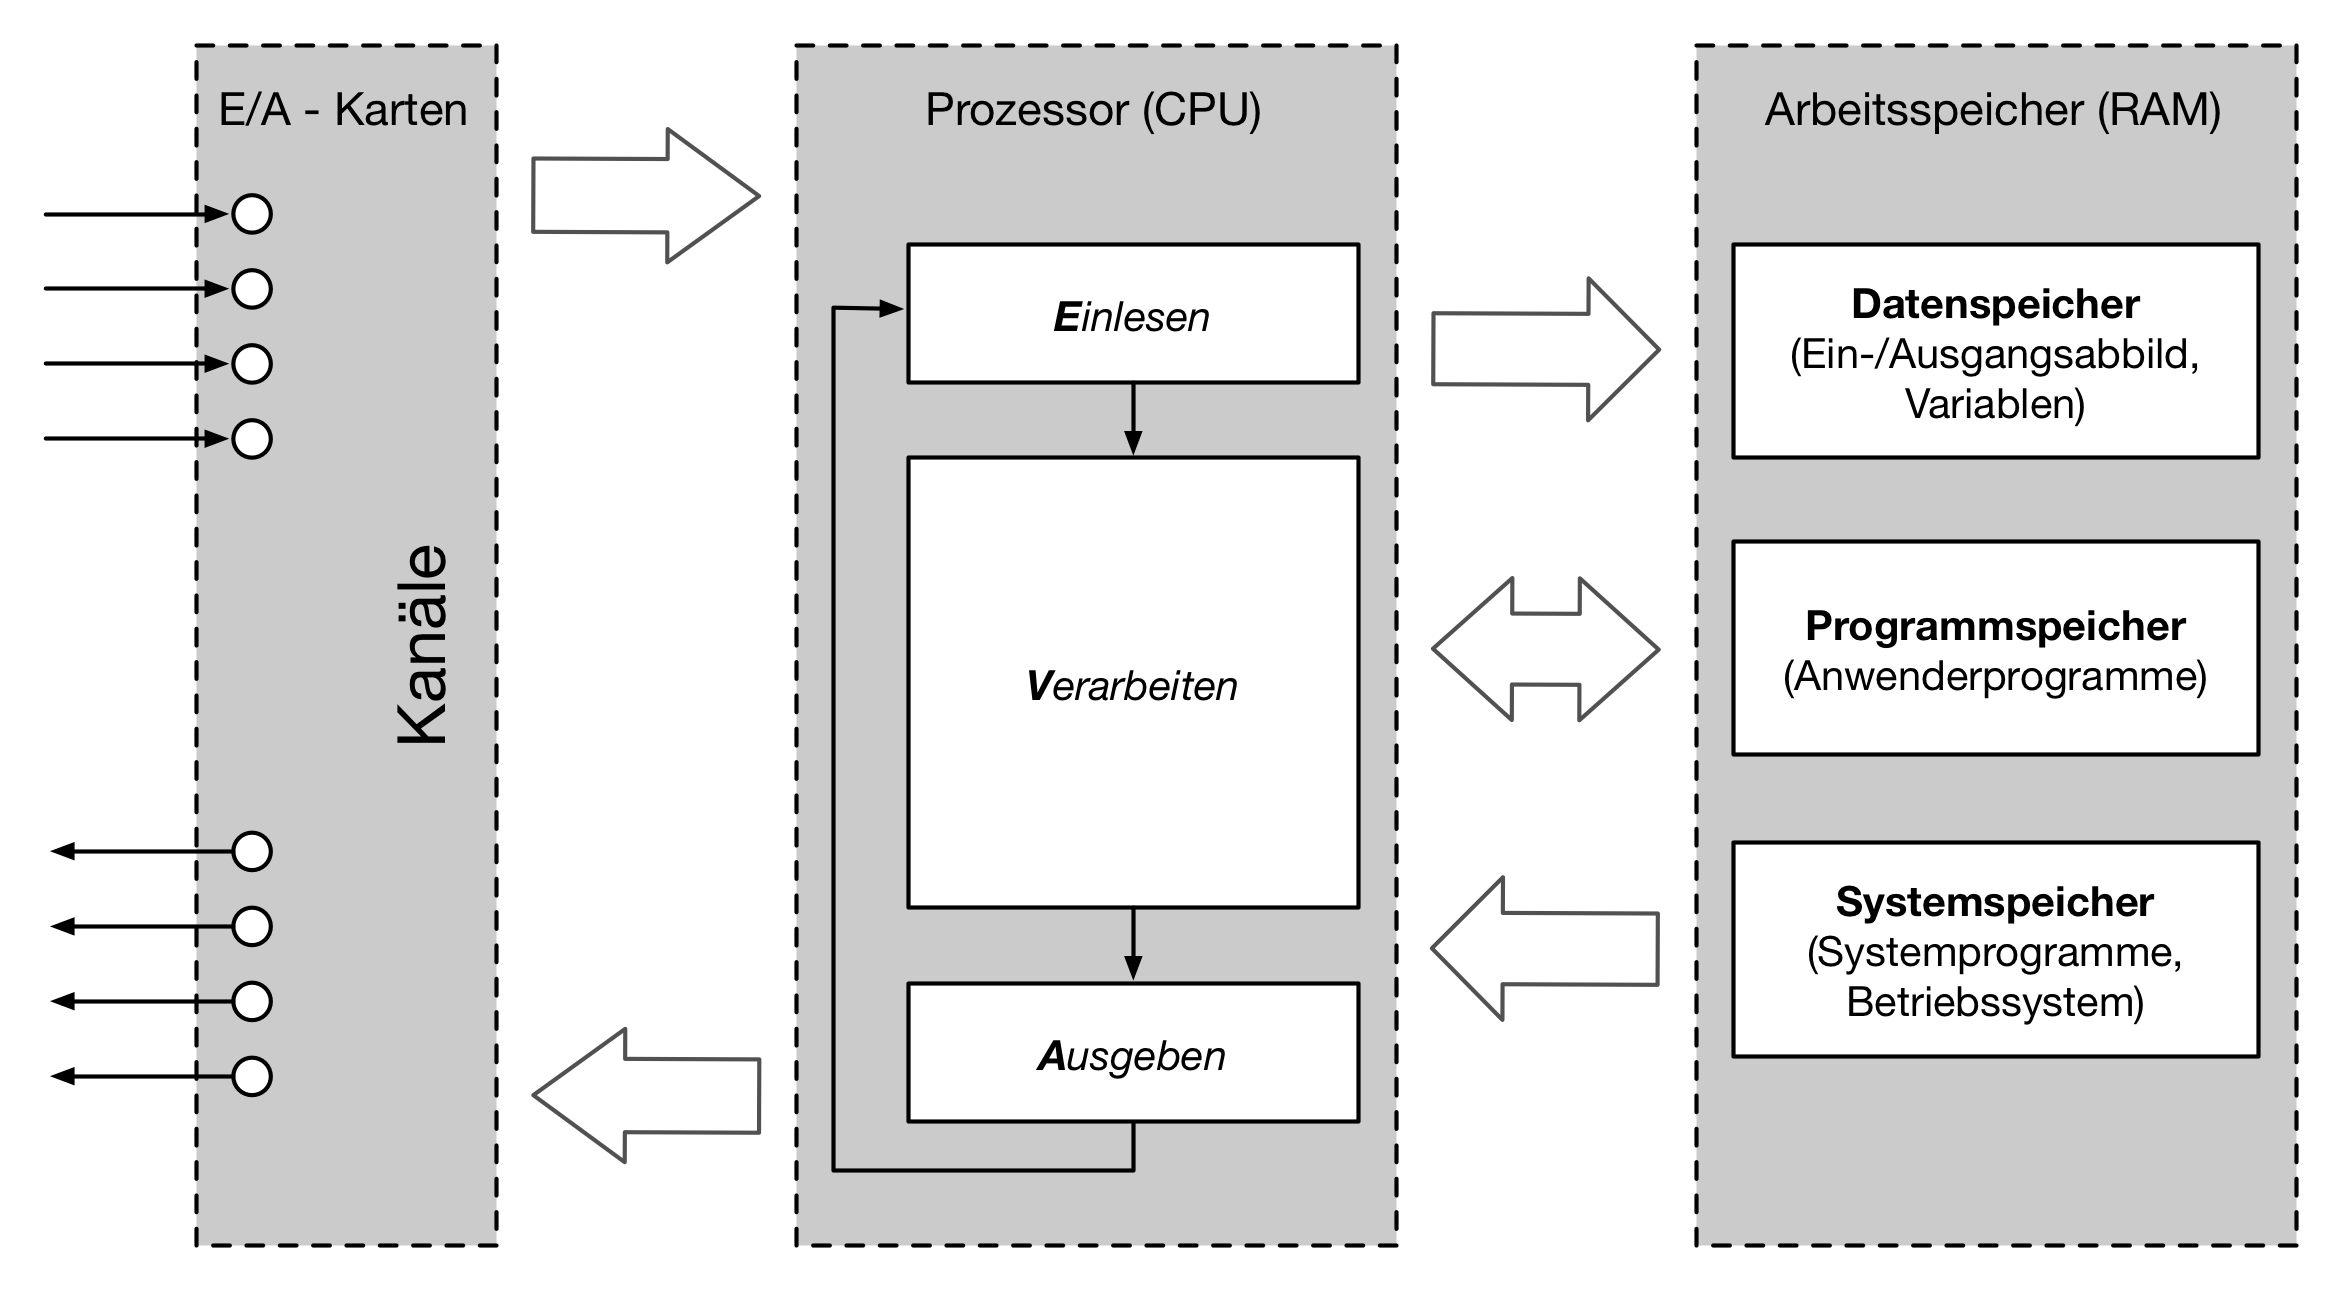
\includegraphics[width=0.7\textwidth]{graphics/stateoftheart/Signalverarbeitung_Selfmade.png}
  		\caption{Signalverarbeitung und Arbeitsweise einer SPS}
	\end{figure}
	
	Kleinere SPS - Hersteller versuchen ihre eigene Hardware möglichst offen für fremde Software zu produzieren, um mit ihrem Produkt eine möglichst große Zielgruppe anzusprechen. Große Hersteller hingegen möchten ihr System eher geschlossen für den Zugriff mittels fremder Software halten, um die Kundenbindung auf den verschiedensten Ebenen der Automatisierungspyramide zu erhöhen.
	
	% ##############################################################
	% Programmierung einer SPS - Wie funktioniert das grundsätzlich?
	% ##############################################################
	\section{Programmierung einer SPS}

	In der Automatisierungs- und Regelungstechnik gibt es zum Erfüllen der gegebenen Anforderung mehrere Wege um diese zu lösen. Genauer gesagt handelt es sich hierbei um ganze sechs verschiedene Programmiersprachen, um auf jede möglich auftretende, sowie spezifische Anforderung individuell eingehen zu können. Diese unterteilen sich wiederum in zwei differenzierbare Untergruppen. So gibt es zum einen die textbasierten Programmiersprachen
	
	\begin{itemize}
		\item[a)] Anweisungsliste (engl. \textit{Instruction List})
		\item[b)] Strukturierter Text (engl. \textit{Structured Text})
		\item[c)] Ablaufsprache (engl. \textit{Sequential Function Chart})
	\end{itemize}

	Im Gegensatz dazu gibt es noch die grafikbasierten Programmiersprachen
	
	\begin{itemize}
		\item[d)] Kontaktplan (engl. \textit{Ladder Diagram})
		\item[e)] Ablaufsprache (engl. \textit{Sequential Function Chart})
		\item[f)] Funktionsbausteinsprache (engl. \textit{Function Block Diagram})
	\end{itemize}
	
	Ziel dieser Vielfalt ist es, eine Vereinheitlichung der Programmierung von SPSen zu erreichen. Der Standard 61131 ist seit 1993 eingeführt und industriell etabliert. Mittlerweile schon in der dritten Edition verfügbar, und somit auch Objektorientierung unterstützend, sind die Programmiersprachen für zentrale \& eng gekoppelte Systeme ausgelegt.\\
	
	\textbf{zu a) - Anweisungsliste}\\
	
	Diese textbasierte Programmiersprache nach der Norm IEC DIN EN 61131-3 ist sehr maschinennahe. Vergleicht man die Anweisungsliste aus Abbildung 2.3 mit höheren Programmiersprachen der Informatik, so ist es eine Art Assemblersprache, die normalerweise 1:1 den jeweiligen Maschinencode übersetzt. Es werden die einzelnen Anweisungen in der Reihenfolge geschrieben, wie sie die Maschine (CPU) abarbeiten soll (auch \glqq Stackorientierte Abarbeitung\grqq \space genannt). Ein großer Vorteil gegenüber allen graphischen Programmiersprachen ist die Tatsache, das AWL funktionell über diese hinausgeht, weil beispielsweise ein komplexer Zählvorgang mittels eines Kontaktplans nicht realisierbar sein könnte.	\cite{spslehrgang_struktur, egroetsch_sps}\\

	\begin{figure}
		\begin{framed}
			VAR\\
			s1: BOOL; \color{gray}//[input] Sensor Deklaration\\ \color{black}
			s2: BOOL; \color{gray}//[input] Sensor Deklaration\\ \color{black}
			s3: BOOL; \color{gray}//[input] Sensor Deklaration\\ \color{black}
			M: BOOL := 0; \color{gray}//[output] Motor Deklaration (muss initialisiert werden)\\ \color{black}
			END\_VAR\\\\
			LD s1; \color{gray}//[load] Lade den boolean-Wert ins Register\\ \color{black}
			OR s2; \color{gray}//Oder-Verknüpfung mit s1\\ \color{black}
			ANDN s3; \color{gray}//Und-Verknüpfung mit invertiertem Eingang\\ \color{black}
			ST \color{gray}//[store] Ergebnis wird in die Variable Motor geschrieben\\
		\end{framed}
		\caption{Beispiel einer Anweisungsliste}
	\end{figure}
	
	\color{black}
	\textbf{zu b) - Strukturierter Text}\\
	
	Diese in Abbildung 2.4 angeführte Programmiersprache der Automatisierungstechnik orientiert sich an der Sprache Pascal, enthält aber neben dieser Sprache zugehörigen spezifischen Elementen aber auch noch SPS-typische Elemente. Geeignet ist ST am vorteilhaftesten für Aufgaben mit mathematischem Hintergrund, sowie zum Beschreiben komplexer Algorithmen. Auch für Rezept- und Datenverwaltung hebt sich diese Art der Programmierung durch enorme Vereinfachung vor. Typische Anweisungen für ST sind solche, die in höheren Sprachen durch Bedingungen oder Schleifen ausgeführt werden können \cite{grundlagen_automatisierungstechnik}\\
	
	\begin{figure}[h]
		\begin{framed}
		\color{black}
		VAR\\
		s1: BOOL; \color{gray}//[input] Sensor Deklaration\\ \color{black}
		s2: BOOL; \color{gray}//[input] Sensor Deklaration\\ \color{black}
		s3: BOOL; \color{gray}//[input] Sensor Deklaration\\ \color{black}
		M: BOOL := 0; \color{gray}//[output] Motor Deklaration ( muss initialisiert werden)\\ \color{black}
		END\_VAR\\
		M := (s1 OR s2) AND ( NOT (s3)); \color{gray}//ODER-Verknüpfung von s1 und s2, anschließendes UND-Verknüpfung von Ergebnis mit negiertem s3.\
		\end{framed}
		\caption{Beispiel eines strukturierten Textes}
	\end{figure}
	\todo[inline]{Schauen ob die Figur \glqq Strukturierter Text\grqq \space an der richtigen Position ist.}
	
	\newpage
	\color{black}
	\textbf{zu c, e) - Ablaufsprache}\\
	
	Eine Sonderstellung unter den Sprachen zur Programmierung einer SPS nimmt die Ablaufsprache ein. \\
	\todo[inline]{Ablaufsprache noch genauer beschreiben!}
	\textbf{zu d) - Kontaktplan}\\
	Die Darstellungsart des Kontaktplans ermöglicht SPS-Programmierern ein Programm auf graphischer Ebene zu erstellen und darzustellen. Ein KOP ist einem Stromlaufplan sehr ähnlich, um Programmieranfängern, die beispielsweise nur in der Elektronik tätig sind/waren und noch nie zuvor analytisch hinterfragten Code entwickelt haben, dein Einstieg zu erleichtern. Es werden Elemente wie Spulen, Öffner/Schließer, Eingänge/Ausgänge, usw... verwendet, die zu logischen Blöcken zusammengefasst werden können und so einen Teil des gesamten Programms ergeben. Ein Nachteil dieser standardisierten Programmiersprache ist jedoch, dass es nicht für alle möglichen Operationen auch ein einheitliches Symbol in einem Stromlaufplan gibt. Das wiederum bedeutet, dass bei komplexen Steuerungen oft eine Mischung aus KOP und der Funktionsbausteinsprache (FBS) verwendet wird.\\
	
	\todo[inline]{Schauen ob das Bild \glqq kop\_Selfmade\grqq \space an der richtigen Position ist.}
	\begin{figure}[h!]
  		\centering
    	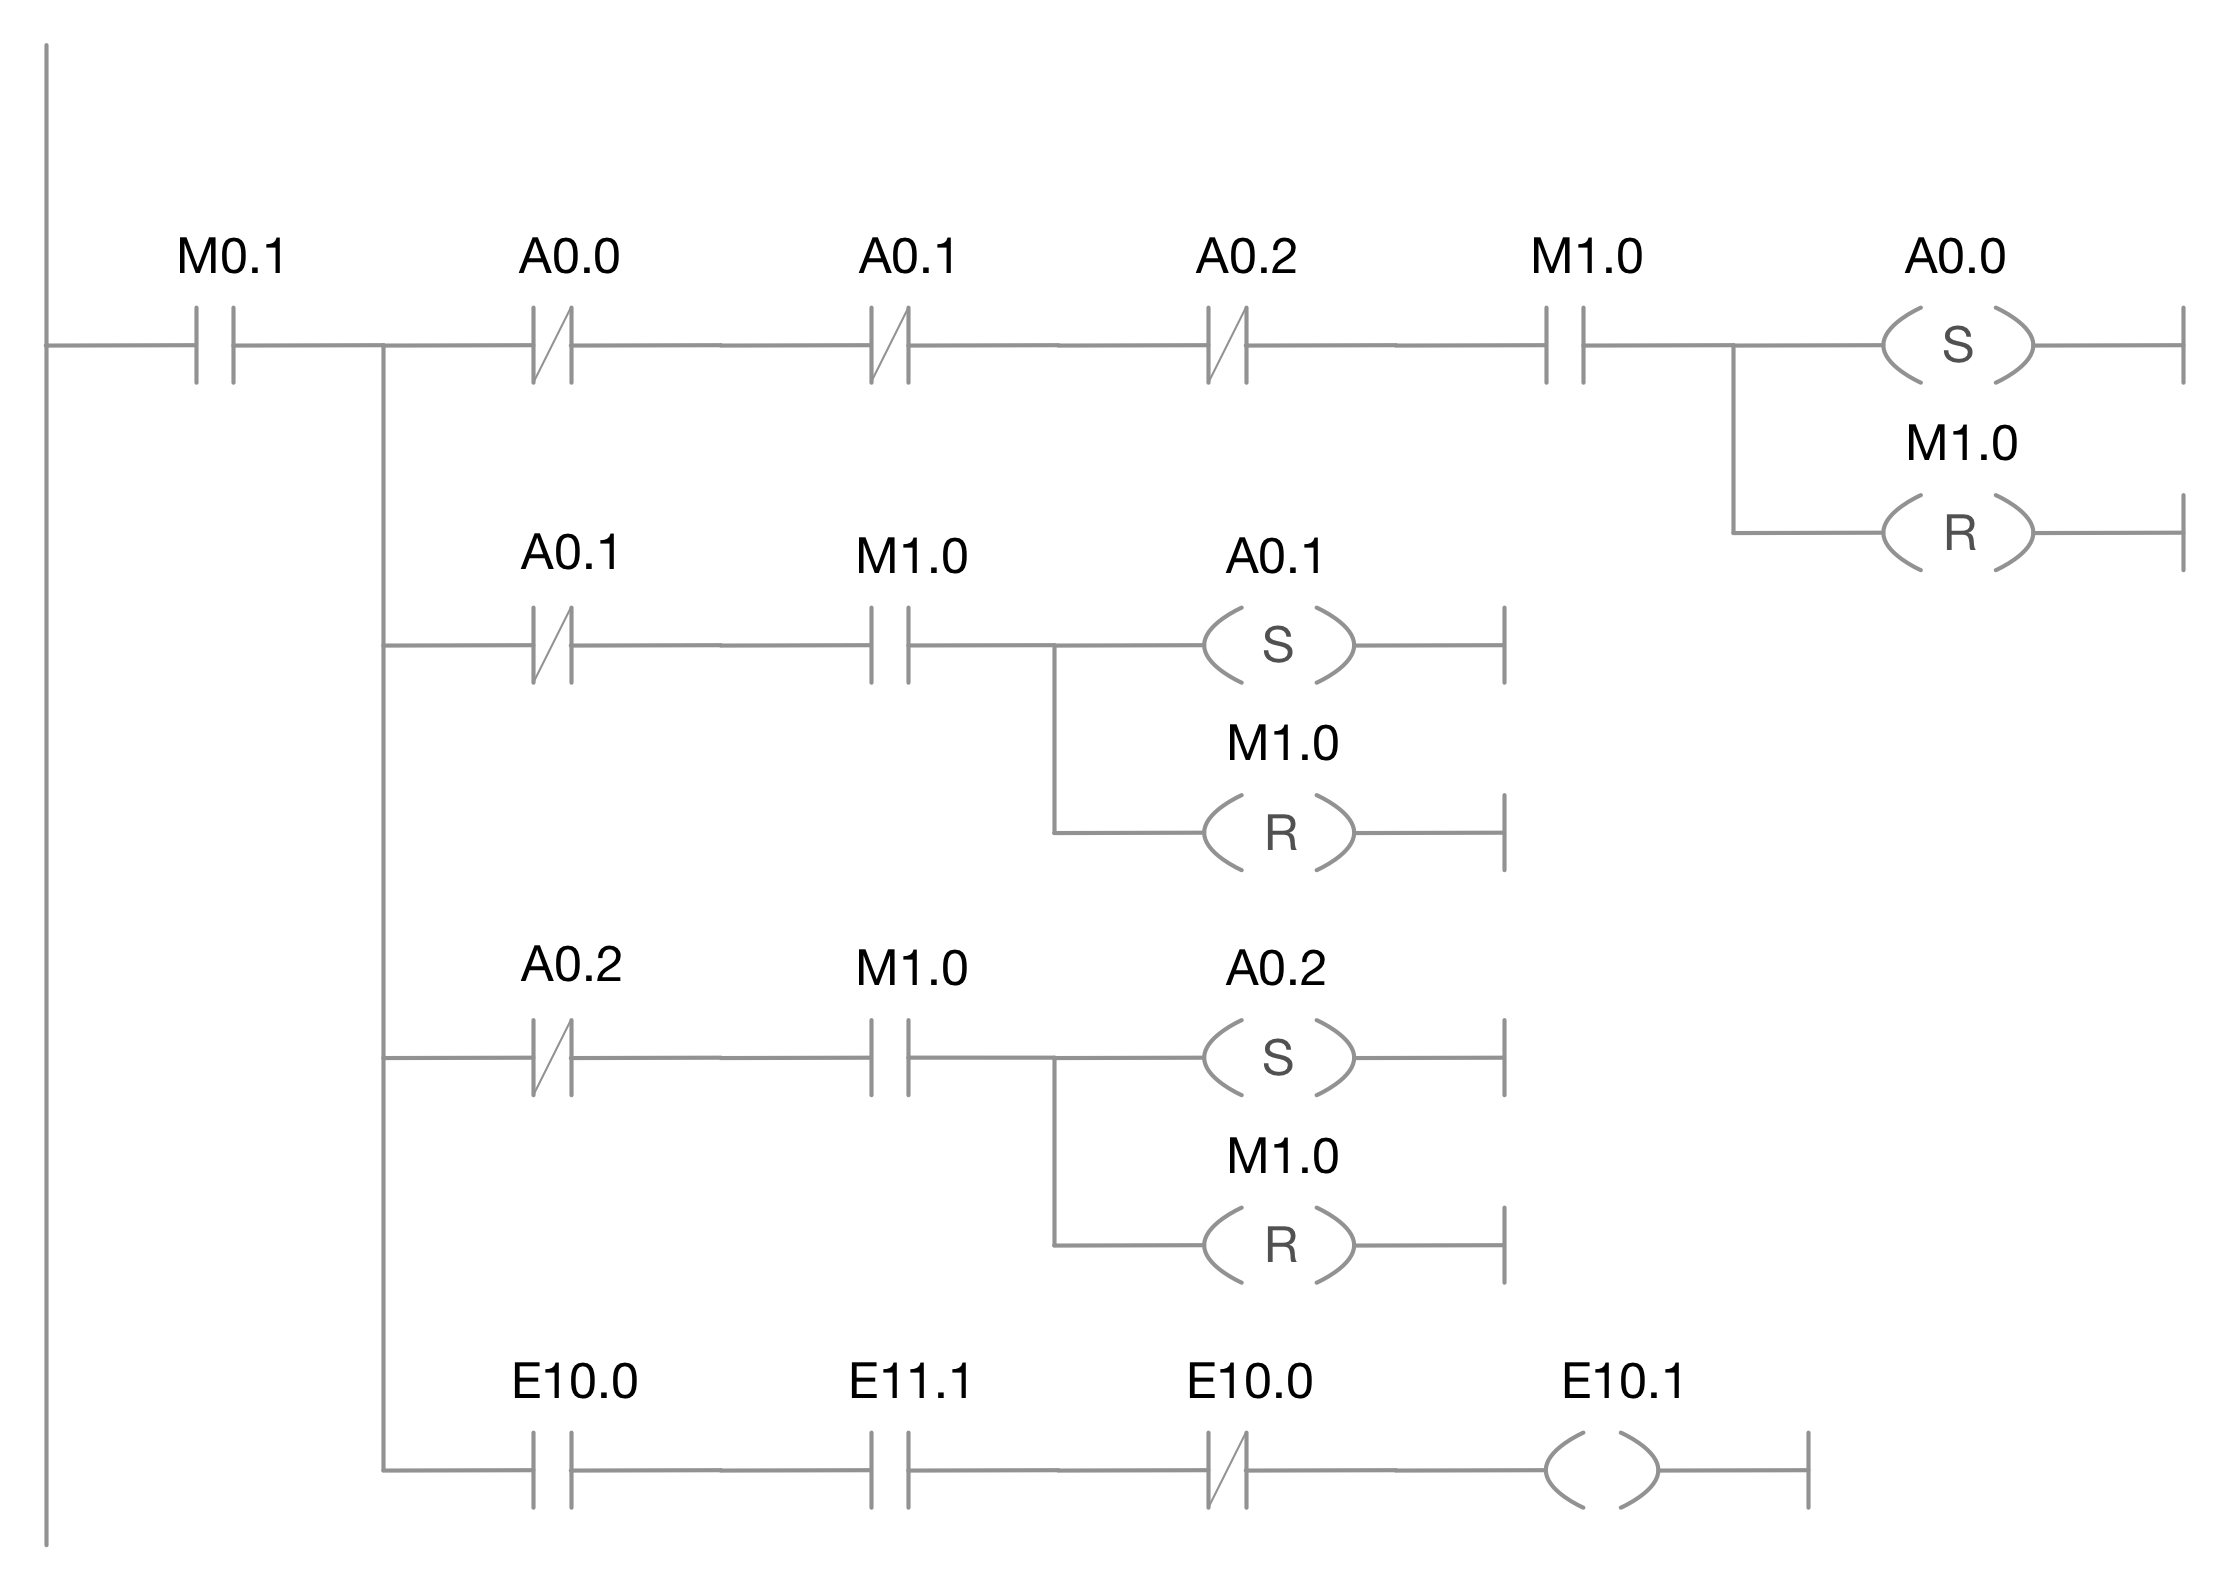
\includegraphics[width=0.55\textwidth]{graphics/stateoftheart/kop_Selfmade.png}
  		\caption{Beispiel eines Kontaktplans}
	\end{figure}

	\newpage
	\textbf{zu f) - Funktionsbausteinsprache}\\

	Diese graphische Programmiersprache verwendet für ihre Anweisungen logische Symbole der Boolschen Algebra. Insbesondere ist diese Sprache für Verknüpfungssteuerungen geeignet und vorallem bei Anfängern oder Nicht-Programmierern beliebt. Durch den einfachen graphischen Aufbau ist die Programmlogik relativ schnell zu erkennen und nachzuvollziehen.

	\textbf{Beispiel eines Funktionsbausteinsplans}	\\
	\begin{figure}[h!]
  		\centering
    	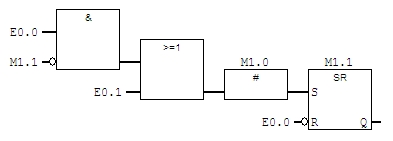
\includegraphics[width=0.8\textwidth]{graphics/stateoftheart/funktionsbausteinplan.jpg}
  		\caption{Funktionsbausteinplan}
	\end{figure}

\section{Phasen und Rezepte}

TODO

\section{Visualisierung von Produktionsanlagen}
\subsection{Anlagen Visualisierung}
%TODO Anlagen Visualisierung
%Quellen/Bilder für Standardisierte Abbildung von Anlagen
\subsection{SCADA}
(Supervisory Control And Data Acquisition)\\
Ein SCADA System ist im Allgemeinen eine Sammelstelle für alle aus der Anlagen generierten Werte. Diese Daten müssen dann weiterverarbeitet werden um aus ihnen Analysen zu erstellen.\\
\\
Zu den Elemente eines SCADA Systems gehören:\\
\\
%todo Quelle Scada
%http://www.engineersgarage.com/articles/scada-systems?page=1
%10 März 2015
\textbf{SCADA Master Station Computer Systems}\\
Sammelstelle für Echtzeitdaten die von RTUs generiert werden. Meist herkömmliche Computer Hardware.\\
\\
\textbf{Human-Machine Interface}\\
Aus den gesammelten Daten Analysen (Prognosen, Diagnosen) so aufbereiten das sie für den Menschen leicht verständlich dargestellt werden.\\
\\
\textbf{Remote Terminal Units (RTUs)}\\
Sensoren die Physikalische Änderungen in der Anlage mit einem Signalumformer in Elektrische Werte umwandelt. Je nachdem was gemessen werden soll, entstehen Analoge (Füllstand, Helligkeit, Druck, ...) oder Digitale (z.B. Status eines Geräts) Werte.\\

\section{Konzeptioneller Entwurf, Modellbasierte Entwicklung}
Das Gebiet der Modellbasierten Entwicklung bzw. der automatisierten Codegenerierung aus so einem Modell als ganzes kann man nicht wirklich als State of the Art erklären.\\
\\
Wenn man sich jedoch die Gebiete als einzelnes anschaut, erkennt man das diese als einzelnes schon heute im Betrieb eingesetzt werden.
\subsection{Modell}
Ein Modell der gesamten Anlage wird schon im frühen Stadium der Entwicklung in Form eines RI-Fließschemas hergestellt um klar zu definieren welche Bauteile benötigt werden und welches mit welchem Bauteil verbunden ist. Dies ist nur das erste Modell das in der Industrie eingesetzt wird.\\
\\
Oft werden aber mehr Informationen benötigt als im RI-Fließschema abbildbar sind, weswegen man auf eine andere Art umsteigen muss ein Modell abzubilden.\\
Auf die gängigsten Methoden (XML,Ontologie,UML) wird in den nächsten Punkten genauer eingegangen.
\subsubsection{XML}
XML ist eine Standardisierte Sprache in der die meisten Strukturen in irgend einer Form abgebildet werden können. Dieser Aspekt macht es zu einem Universalen Standard der in verschieden Sparten eingesetzt wird.\\
Ein Nachteil von XML ist es, dass es sich hierbei um eine Textuelle Form eines Modells handelt was für Menschen schwerer zu verstehen ist als eine Visuelle Abbildung.\\
Dafür gibt es die nächsten 2 Werkzeuge die beide auf XML basieren.
\subsubsection{Ontologie}
%todo Quelle Ontologie
%http://plato.stanford.edu/entries/logic-ontology/
\begin{displayquote}... we have at least two parts to the overall philosophical project of ontology: first, say what there is, what exists, what the stuff is reality is made out off, secondly, say what the most general features and relations of these things are.
\end{displayquote}
Eine Ontologie ist ein auf XML basierendes Konstrukt das einem das Abbilden von Dingen und deren Relationen ermöglicht. Um solch Komplexe Zustände darzustellen stehen einem neben einfachen Entitäten(Dinge) auch Eigenschaften zur verfügen.\\
\\
\textbf{Allgemeiner Aufbau einer Ontologie}\\
Das Modell an sich ohne zusätzliche Attribute oder Eigenschaften ist vom Aufbau her so zu erklären, dass es ein Thing gibt von dem alles aus geht (Sozusagen der Ursprung von allem). Von diesem Punkt aus können weitere Entitäten abgeleitet werden (Eine Vererbung, vergleichbar mit einem Stammbaum). Die neu erstellte Entität ist immer noch ein Thing, jedoch genauer beschrieben. Diese Vererbung wird dann soweit wie benötigt weitergeführt.\\
%Todo Beispiel Ontologie
%Aufbau Grafik Thing -> Ebene 1 -> Ebene 2...
\\
\textbf{Object Properties}\\
Object Properties sind Eigenschaften die die Relationen zwischen den Einzelnen Objekten/Entitäten genauer beschreiben.\\ 
\\
\textbf{Data Properties}\\
Data Properties sind Eigenschaften die die Entitäten genauer beschreiben bzw. erklären. 
\\
\\
Dies ermöglicht ein Modell aufzubauen das nicht nur Triviale Daten wie: Welche Bauteile gibt es..., abbilden kann, sondern komplexe Strukturen zu konstruieren. Ein Anwendungsfall bei einem Modell für eine Produktionsanlage ist es etwaigen Sensoren direkt im Modell einen Wertebereich festzulegen in dem dieser Sensor arbeitet bzw. Werte liefert, Beispiel hierfür: Ein Füllstandsensor mit einem Wertebereich von 4-20V, wobei 4V=Leer und 20V=Voll bedeutet, kann in einer Ontologie mit wenigen Data Properties abgebildet werden.
\subsubsection{UML}
UML ist eine Methode die in vielen verschiedenen Gebieten Einsatz findet da sie sehr Unabhängig aufgebaut ist. Man kann sowohl in der Softwareentwicklung ganze Programme abbilden als auch eine ganze Produktionsanlage. Anders als bei Ontologien gibt es bei UML jedoch andere Modelle als nur eine Abbilden der Anlage, beispielsweise kann in einem Aktivitätsdiagramm eine Phase oder ein ganzen Rezept abgebildet werden.
\subsection{Automatische Codegenerierung}

TODO

\section{Fazit}

%TODO Codegenerierung
%Sinnvoll in State of the Art?	